\title{\href{http://puredata.info/}{Pure Data}}

\maketitle
\tableofcontents

% http://puredata.info/docs/faq
%http://www.pdpatchrepo.info/hurleur/Spect.pd

\section{About Pure Data}
%{{{

\begin{itemize}
\item Pure Data (Pd) is a interactive real-time graphical programming
  environment for audio, video, and graphical processing.
\item Pd was originally created by \href{http://msp.ucsd.edu/}{Miller
    Puckette} at \href{http://www.ircam.fr/}{IRCAM}.
\item It is written in
  \href{http://en.wikipedia.org/wiki/C_\%28programming_language\%29}{C}
  and \href{http://en.wikipedia.org/wiki/Tcl}{Tcl}.
\item Pd is \href{http://puredata.info/about/pdlicense}{open source}
  and runs on Linux, Windows, Mac Os X and Android.
\end{itemize}

%}}}

\section{Installation (of Pure Data Extended)}
%{{{

\begin{itemize}
\item \href{http://puredata.info/downloads/pd-extended}{Pure Data
    Extended} is an extension (with libraries written by the community
  for graphics rendering (GEM library), OSC communications, binary
  file processing, audio-visual streaming, physical modeling,
  sensor-based performances, etc.) of
  \href{http://puredata.info/downloads/pure-data}{Pure Data Vanilla}.
  \begin{enumerate}
  \item \href{http://puredata.info/docs/faq/macosx}{MacOS X}.
  \item \href{http://puredata.info/docs/faq/debian}{Debian(s)}.
  \item \href{http://puredata.info/docs/faq/redhat}{RedHat}.
  \item \href{http://puredata.info/docs/faq/w32}{Windows}.
  \end{enumerate}
\end{itemize}

%}}}

\section{How to run Pd}
%{{{

\begin{verbatim}
pd-extended &
\end{verbatim}

%}}}

\section{On-line documentation}
%{{{

\begin{itemize}
\item \href{http://puredata.info/docs}{Main Pd documentation}.
\item \href{http://en.flossmanuals.net/PureData/}{Floss Manuals}
\end{itemize}

%}}}

\section{Pd in-place documentation}
%{{{

\begin{itemize}
\item \verb|Pd-extended->Help->Help Browser|.
\item \verb|Pd-extended->Search|.
\item On any object of the canvas, click the righ button of your
  mouse and select ``Help'' to get information about that object.
\end{itemize}

%}}}

\section{I want even more (external) libraries!}
%{{{

\begin{enumerate}
\item
  \href{http://puredata.info/downloads/by-category/library}{Projects
    In Category Libraries And Externals}.
\item
  \href{http://puredata.info/community/member-downloads/patches}{Pd
    Patches}.
\end{enumerate}

%}}}

\section{\href{http://puredata.info/docs/developer/PdFileFormat}{Patches, objects, wires, ...}}
%{{{

\begin{enumerate}
\item A {\bf patch} is a collection of Pd {\bf elements} (usually
  stored in a {\tt .pd} file).
\item Elements of a patch are {\bf objects} that have been already
  placed in a patch (at least have size and position in the {\bf
    canvas}).
\item {\bf Wires} transport {\bf messages} between objects.
\end{enumerate}

%}}}

\section{(Some of the) Supported Inputs/Outputs}
%{{{

\begin{enumerate}
\item \href{http://en.flossmanuals.net/pure-data/ch079_audio-glue/}{PCM audio}.
\begin{verbatim}
cat > ADC-DAC.pd << EOF
#N canvas 596 824 450 300 10;
#X obj 117 84 adc~;
#X obj 118 113 dac~;
#X text 43 98 Left channel;
#X text 147 99 Right channel;
#X text 149 84 Read audio from the Analog-to-Digital Converter;
#X text 149 113 Write audio to the Digital-to-Analog Converter;
#X connect 0 0 1 0;
#X connect 0 1 1 1;
EOF

pd-extended ADC-DAC.pd &

# Remember to activate DSP in the Pd main window!
\end{verbatim}

\begin{center}
  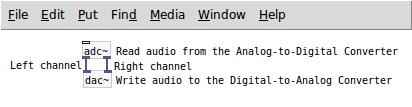
\includegraphics{ADC-DAC}
  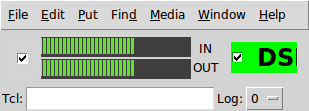
\includegraphics{ADC-DAC-pd}
  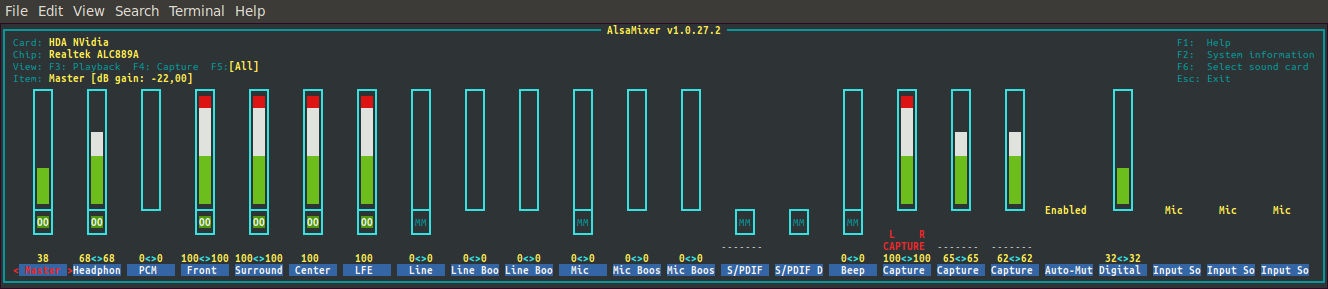
\includegraphics{ADC-DAC-alsamixer}
  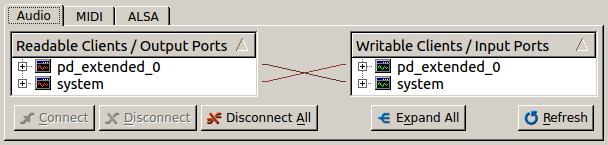
\includegraphics{ADC-DAC-jack-Audio}
\end{center}

\item
  \href{http://en.flossmanuals.net/pure-data/midi/using-midi/}{MIDI}. Run
  \texttt{qjacktcl}, \texttt{vmpk}, \texttt{amsynth} and connect in
  the ALSA Connections facility ``VMPK Output'' with ``Pure Data''
  and``Pure Data'' with ``amSynth''.
\begin{verbatim}
cat > MIDI-IO.pd << EOF
#N canvas 962 48 956 1131 10;
#X obj 33 23 notein;
#X obj 27 107 noteout;
#X text 72 85 <- MIDI channel number;
#X text 37 51 <------- Note number;
#X text 54 68 <---- Velocity;
#X text 82 23 Read note;
#X text 81 107 Write note;
#X connect 0 0 1 0;
#X connect 0 1 1 1;
#X connect 0 2 1 2;
EOF

pd-extended MIDI-IO.pd &

% Remember to select "jack" and "ALSA-MIDI" in Pd!
\end{verbatim}

\begin{center}
  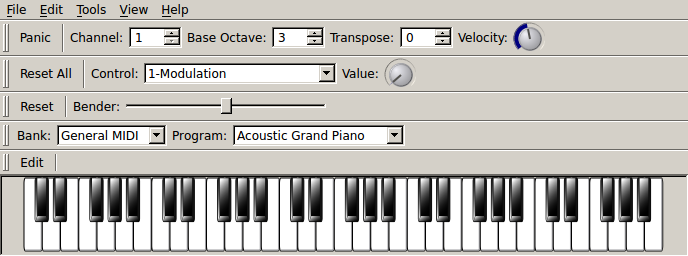
\includegraphics{VMPK}
  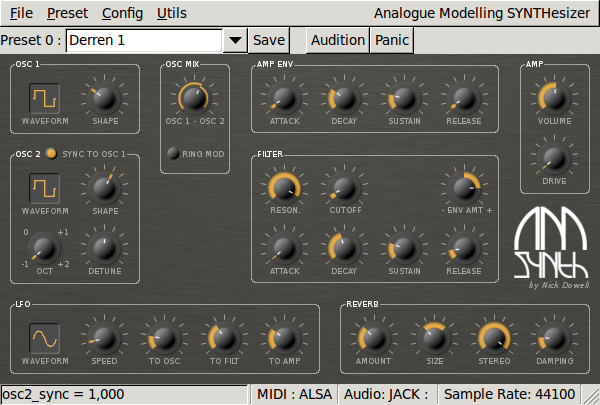
\includegraphics{AMSynth}
  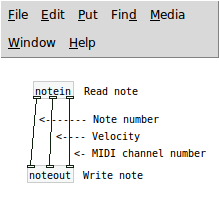
\includegraphics{MIDI-IO}
  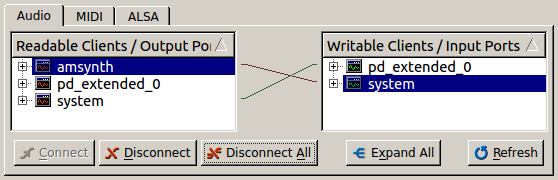
\includegraphics{MIDI-IO-jack-Audio}
  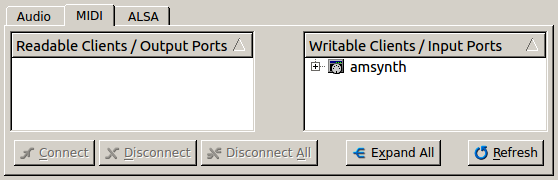
\includegraphics{MIDI-IO-jack-MIDI}
  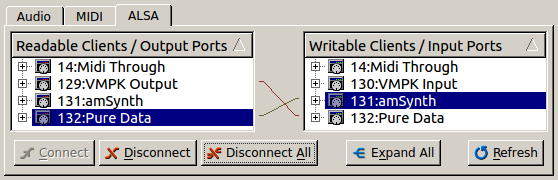
\includegraphics{MIDI-IO-jack-ALSA}
\end{center}

\item \href{http://en.flossmanuals.net/pure-data/ch049_moving-images/}{Video}.
\begin{verbatim}
cat > webcam.pd << EOF
#N canvas 92 850 450 300 10;
#X obj 117 91 gemhead;
#X msg 149 117 device 0;
#X obj 124 147 pix_video;
#X obj 230 157 gemwin;
#X obj 124 169 pix_texture;
#X obj 124 191 rectangle 6 4;
#X msg 231 134 dimen 640 480 \, create \, 1;
#X connect 0 0 2 0;
#X connect 1 0 2 0;
#X connect 2 0 4 0;
#X connect 4 0 5 0;
#X connect 6 0 3 0;
EOF

pd-extended webcam.pd &

% A window named GEN should be created with the video captured by the webcam.
\end{verbatim}

\begin{center}
  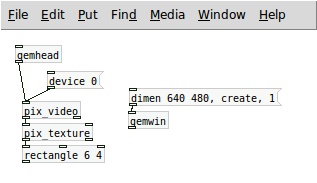
\includegraphics{webcam}
\end{center}

\item \href{http://en.flossmanuals.net/pure-data/ch056_game-controllers/}{Keyboard}.
\begin{verbatim}
cat > keyboard.pd << EOF
#N canvas 80 659 450 300 10;
#X obj 59 28 key;
#X floatatom 59 51 5 0 0 0 - - -;
#X connect 0 0 1 0;
EOF

pd-extended keyboard.pd &

% After selecting the window, push any key.
\end{verbatim}

\begin{center}
  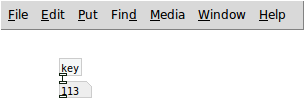
\includegraphics{keyboard}
\end{center}

\item \href{http://en.flossmanuals.net/pure-data/ch056_game-controllers/}{Mouse}.
\begin{verbatim}
cat > mouse.pd << EOF
#N canvas 82 473 450 300 10;
#X obj 135 72 cursor;
#X obj 135 54 tgl 15 0 empty empty empty 17 7 0 10 -262144 -1 -1 1
1;
#X obj 135 93 route motion;
#X obj 135 115 route x y;
#X floatatom 119 143 5 0 0 0 - - -;
#X floatatom 173 142 5 0 0 0 - - -;
#X obj 135 169 osc~;
#X obj 167 169 osc~;
#X obj 145 196 dac~;
#X text 152 141 x;
#X text 208 139 y;
#X connect 0 0 2 0;
#X connect 1 0 0 0;
#X connect 2 0 3 0;
#X connect 3 0 4 0;
#X connect 3 1 5 0;
#X connect 4 0 6 0;
#X connect 5 0 7 0;
#X connect 6 0 8 0;
#X connect 7 0 8 1;
EOF

pd-extended mouse.pd &

# Activate the patch and the DSP, and move the mouse!
\end{verbatim}

\begin{center}
  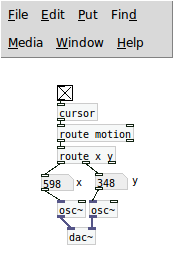
\includegraphics{mouse}
  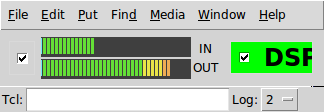
\includegraphics{mouse-pd}
  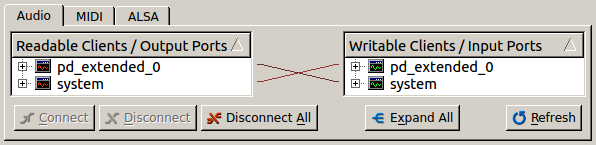
\includegraphics{mouse-jack}
\end{center}

\item \href{http://en.flossmanuals.net/pure-data/ch056_game-controllers/}{USB HID}.

\begin{verbatim}
# Before running pd, plug the device!

cat > hid.pd << EOF
#N canvas 1396 119 176 115 10;
#X msg 90 15 print;
#X obj 51 43 hid;
#X obj 51 72 print;
#X obj 19 16 tgl 15 0 empty empty empty 17 7 0 10 -262144 -1 -1 1 1
;
#X msg 40 15 open 8;
#X connect 0 0 1 0;
#X connect 1 0 2 0;
#X connect 3 0 1 0;
#X connect 4 0 1 0;
EOF

pd-extended hid.pd &

# Don't forget to: (1)  toggle on the patch, (2) send the "print" message
# to the "hid" object, (3) send the right "open" to the right device.
\end{verbatim}

\begin{center}
  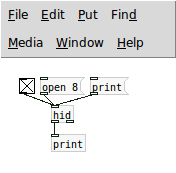
\includegraphics{hid}
  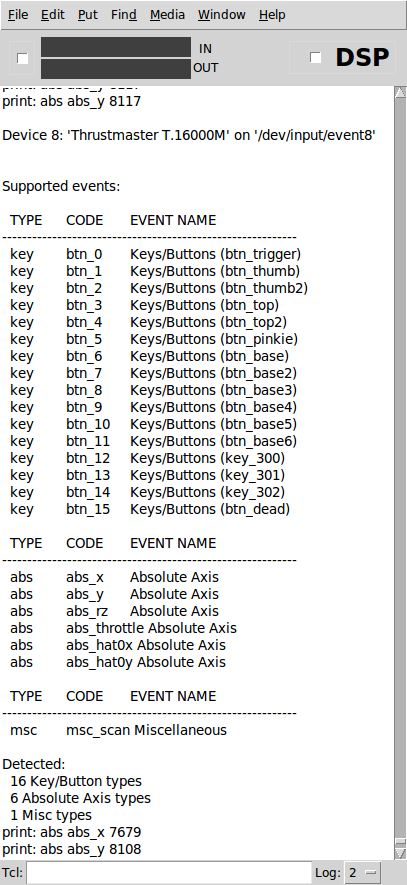
\includegraphics{hid-pd}
\end{center}

\end{enumerate}

%}}}

\section{A MIDI music random generator}
%{{{

%\begin{itemize}
%\item To test this patch, run the following programs:
%  \begin{enumerate}
%  \item {\tt qjackctl} and start the daemon.
%  \item {\tt amsynth} and check if the MIDI writable client ``amsynth''
%    appears and if the ALSA writable client ``amSynth'' also appears.
%  \item {\tt pd-extended} and select ``jack'' and ``ALSA-MIDI'' in the
%    ``Media'' menu.
%  \end{enumerate}
%\end{itemize}
\begin{verbatim}
cat > MIDI-random-generator.pd << EOF
#N canvas 2 48 476 1131 10;
#X obj 35 114 drunk 10;
#X floatatom 35 169 5 0 0 0 - - -;
#X obj 35 35 metro 300;
#X obj 35 12 tgl 15 0 empty empty empty 0 -6 0 8 -262144 -1 -1 0 1
;
#X floatatom 57 63 5 0 0 0 - - -;
#X floatatom 80 87 5 0 0 0 - - -;
#X floatatom 86 15 5 0 0 0 - - -;
#X obj 35 140 + 21;
#X text 114 84 Step size;
#X text 90 61 Upper bound;
#X obj 38 191 hsl 128 15 21 108 0 0 empty empty empty -2 -8 0 10 -262144
-1 -1 2628 1;
#X obj 377 42 ctlout 1;
#X floatatom 377 17 0 0 0 0 - - -;
#X obj 35 254 makenote;
#X floatatom 57 215 5 0 0 0 - - -;
#X floatatom 80 234 5 0 0 0 - - -;
#X obj 118 293 noteout 1;
#X obj 187 116 drunk 10;
#X floatatom 187 171 5 0 0 0 - - -;
#X obj 187 37 metro 300;
#X obj 187 14 tgl 15 0 empty empty empty 0 -6 0 8 -262144 -1 -1 0 1
;
#X floatatom 209 65 5 0 0 0 - - -;
#X floatatom 232 89 5 0 0 0 - - -;
#X floatatom 238 17 5 0 0 0 - - -;
#X obj 187 142 + 21;
#X text 266 86 Step size;
#X text 242 63 Upper bound;
#X obj 190 193 hsl 128 15 21 108 0 0 empty empty empty -2 -8 0 10 -262144
-1 -1 292 1;
#X obj 187 256 makenote;
#X floatatom 209 217 5 0 0 0 - - -;
#X floatatom 232 236 5 0 0 0 - - -;
#X text 122 16 Period;
#X text 273 18 Period;
#X text 218 141 MIDI notes start at 21;
#X text 242 218 Velocity;
#X text 266 237 Duration (ms);
#X connect 0 0 7 0;
#X connect 1 0 10 0;
#X connect 2 0 0 0;
#X connect 3 0 2 0;
#X connect 4 0 0 1;
#X connect 5 0 0 2;
#X connect 6 0 2 1;
#X connect 7 0 1 0;
#X connect 10 0 13 0;
#X connect 12 0 11 0;
#X connect 13 0 16 0;
#X connect 13 1 16 1;
#X connect 14 0 13 1;
#X connect 15 0 13 2;
#X connect 17 0 24 0;
#X connect 18 0 27 0;
#X connect 19 0 17 0;
#X connect 20 0 19 0;
#X connect 21 0 17 1;
#X connect 22 0 17 2;
#X connect 23 0 19 1;
#X connect 24 0 18 0;
#X connect 27 0 28 0;
#X connect 28 0 16 0;
#X connect 28 1 16 1;
#X connect 29 0 28 1;
#X connect 30 0 28 2;
EOF

pd-extended MIDI-random-generator.pd &

# Ensure that "jack" and "ALSA-MIDI" have been selected in the "Media" menu.
\end{verbatim}

\begin{center}
  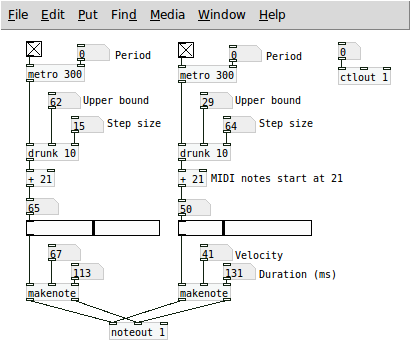
\includegraphics{MIDI-random-generator}
  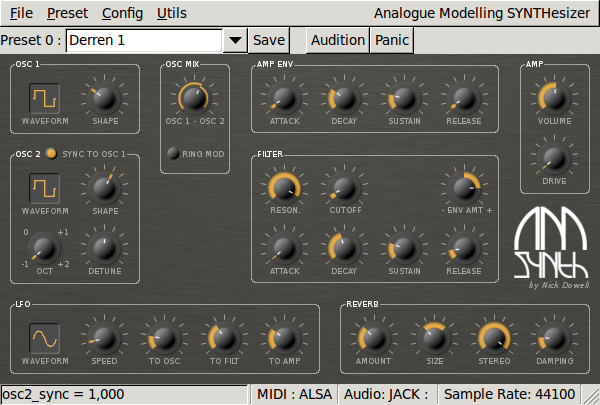
\includegraphics{MIDI-random-generator-amsynth}
  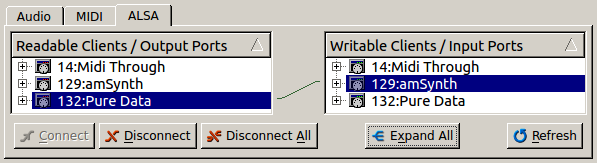
\includegraphics{MIDI-random-generator-jack-ALSA}
\end{center}

%}}}

\section{An amplitude (audio) modulator}
\begin{itemize}
\item Version 1:
\begin{verbatim}
cat > amplitude-modulation-1.pd << EOF
#N canvas 907 133 949 688 10;
#X obj 96 53 adc~;
#X obj 347 149 *~;
#X obj 379 148 *~;
#X obj 365 196 dac~;
#X obj 369 85 osc~;
#X obj 80 156 env~;
#X obj 129 156 env~;
#X obj 81 219 vu 15 120 empty empty -1 -8 0 10 -66577 -1 1 0;
#X obj 130 218 vu 15 120 empty empty -1 -8 0 10 -66577 -1 1 0;
#X obj 129 194 - 100;
#X obj 80 195 - 100;
#X obj 26 -65 tgl 15 0 empty empty empty 17 7 0 10 -262144 -1 -1 1
1;
#X msg 26 -45 \; pd dsp \$1;
#X obj 225 400 tabwrite~ R-wave;
#X obj 22 401 tabwrite~ L-wave;
#N canvas 0 0 450 300 (subpatch) 0;
#X array L-wave 100 float 3;
#A 0 7.15256e-07 -2.38419e-07 3.8147e-06 -8.34465e-07 3.57628e-06 1.43051e-06
-2.26498e-06 2.86102e-06 -1.90735e-06 -2.86102e-06 1.19209e-07 -4.76837e-07
-4.29153e-06 8.34465e-07 1.19209e-06 -5.96047e-07 2.14577e-06 -1.66893e-06
4.76837e-07 5.84126e-06 -2.02656e-06 -2.74181e-06 3.21865e-06 -1.07288e-06
3.57628e-06 2.02656e-06 -3.69549e-06 -1.19209e-07 -5.96047e-07 -1.78814e-06
-1.07288e-06 -9.53674e-07 -4.17233e-06 -7.39098e-06 -1.54972e-06 -3.33786e-06
-2.38419e-07 -6.07967e-06 -3.45707e-06 -1.19209e-07 -2.6226e-06 -1.66893e-06
-3.57628e-07 9.53674e-07 0 -2.5034e-06 -3.09944e-06 -7.15256e-07 -4.29153e-06
-6.67572e-06 3.45707e-06 -8.34465e-07 -2.38419e-06 -2.02656e-06 -3.45707e-06
-5.96047e-07 -1.19209e-06 -2.38419e-07 -9.53674e-07 -9.53674e-07 -9.53674e-07
-1.19209e-07 5.96047e-07 -2.74181e-06 -5.96047e-07 -3.45707e-06 -4.76837e-06
-2.5034e-06 -6.07967e-06 -1.01328e-05 -5.96047e-06 -6.31809e-06 -5.72205e-06
-5.126e-06 -1.00136e-05 -8.22544e-06 -6.67572e-06 -9.05991e-06 -6.79493e-06
-5.84126e-06 -7.15256e-06 -8.34465e-06 -3.33786e-06 -4.41074e-06 -3.33786e-06
-6.55651e-06 -4.52995e-06 3.21865e-06 -5.00679e-06 -4.41074e-06 -1.78814e-06
-2.98023e-06 -3.21865e-06 -5.96047e-06 -2.5034e-06 2.26498e-06 -1.78814e-06
-7.98702e-06 -7.15256e-07 -1.54972e-06;
#X coords 0 1 99 -1 200 140 1;
#X restore 22 437 graph;
#N canvas 0 0 450 300 (subpatch) 0;
#X array R-wave 100 float 3;
#A 0 -2.38419e-07 -1.54972e-06 2.74181e-06 2.38419e-07 5.96047e-07
-2.02656e-06 -3.21865e-06 -2.14577e-06 -2.5034e-06 -3.93391e-06 -3.93391e-06
1.90735e-06 -3.45707e-06 -5.126e-06 -1.07288e-06 -5.96047e-07 0 -2.5034e-06
-2.6226e-06 2.74181e-06 2.6226e-06 -5.24521e-06 -3.57628e-07 3.57628e-06
-5.96047e-07 5.96047e-07 4.76837e-07 -2.02656e-06 5.96047e-07 -4.64916e-06
-2.6226e-06 -3.45707e-06 -4.52995e-06 -5.84126e-06 -4.88758e-06 -6.55651e-06
-2.5034e-06 -6.31809e-06 -5.84126e-06 -1.43051e-06 -5.96047e-06 -5.36442e-06
-5.00679e-06 -4.88758e-06 -3.45707e-06 -7.6294e-06 -6.19888e-06 -4.64916e-06
-4.41074e-06 -2.98023e-06 -3.45707e-06 -1.54972e-06 -5.60284e-06 -8.34465e-07
-1.43051e-06 3.33786e-06 -3.57628e-07 -4.88758e-06 1.43051e-06 2.14577e-06
-4.76837e-07 -1.3113e-06 4.17233e-06 1.19209e-06 -1.78814e-06 -2.74181e-06
-6.79493e-06 -1.3113e-06 -3.21865e-06 -9.29833e-06 8.34465e-07 -4.76837e-06
-9.05991e-06 -8.22544e-06 -6.91414e-06 -2.38419e-06 -5.48363e-06 -9.41753e-06
-7.03335e-06 -4.76837e-06 -3.33786e-06 -5.48363e-06 -5.84126e-06 -6.31809e-06
-2.86102e-06 -7.6294e-06 -3.8147e-06 -2.5034e-06 -4.64916e-06 3.57628e-07
-1.07288e-06 -2.02656e-06 -4.52995e-06 -1.90735e-06 -1.07288e-06 -1.90735e-06
-1.3113e-06 -5.84126e-06 1.43051e-06 3.33786e-06;
#X coords 0 1 99 -1 200 140 1;
#X restore 225 437 graph;
#X obj 348 243 tgl 15 0 empty empty empty 17 7 0 10 -262144 -1 -1 1
1;
#X obj 535 -1 rfft~;
#X obj 525 27 *~;
#X obj 567 26 *~;
#X obj 537 63 sqrt~;
#X obj 522 101 tabwrite~ L-spectrum;
#X obj 736 -2 rfft~;
#X obj 726 26 *~;
#X obj 768 25 *~;
#X obj 738 62 sqrt~;
#X obj 725 100 tabwrite~ R-spectrum;
#N canvas 0 0 450 300 (subpatch) 0;
#X array L-spectrum 32 float 5;
#A 0 5.71013e-05 4.32817e-05 1.20384e-05 3.48559e-05 8.77849e-06 2.19825e-05
4.74943e-06 1.30174e-05 1.16016e-05 1.52102e-05 1.47943e-05 6.02108e-06
2.82748e-05 8.00954e-06 1.33847e-05 1.26131e-05 2.90345e-05 1.71747e-05
1.99527e-05 8.0148e-06 5.46966e-06 2.88755e-05 3.64437e-05 3.49496e-05
1.23923e-05 1.35475e-05 1.38634e-05 1.89308e-05 2.77127e-05 7.08749e-06
1.0293e-05 4.91514e-06;
#X coords 0 1 31 -1 200 140 1;
#X restore 522 137 graph;
#N canvas 0 0 450 300 (subpatch) 0;
#X array R-spectrum 32 float 5;
#A 0 0.000133872 6.65336e-05 6.16975e-05 2.6333e-05 9.60711e-06 1.8283e-05
1.49031e-06 2.69171e-06 3.37218e-06 1.02522e-05 1.5449e-05 1.41368e-05
3.5513e-06 1.65844e-05 1.12967e-06 2.44163e-05 4.74706e-05 4.18902e-06
2.01457e-05 1.39197e-05 1.69537e-05 1.80982e-05 1.03847e-05 3.24139e-05
1.43496e-05 7.90919e-06 1.31608e-05 1.36888e-05 1.7326e-05 1.23782e-05
1.87602e-05 7.10071e-06;
#X coords 0 1 31 -1 200 140 1;
#X restore 725 137 graph;
#X obj 535 304 rfft~;
#X obj 525 332 *~;
#X obj 567 331 *~;
#X obj 537 368 sqrt~;
#N canvas 0 0 450 300 (subpatch) 0;
#X array L-spectrum-m 32 float 1;
#A 0 2.25592e-05 1.70995e-05 4.75608e-06 1.37706e-05 3.46815e-06 8.6847e-06
1.87638e-06 5.14285e-06 4.58351e-06 6.00916e-06 5.84484e-06 2.37877e-06
1.11706e-05 3.16436e-06 5.28796e-06 4.9831e-06 1.14708e-05 6.78528e-06
7.88281e-06 3.16644e-06 2.16092e-06 1.1408e-05 1.4398e-05 1.38077e-05
4.89589e-06 5.35226e-06 5.47708e-06 7.47908e-06 1.09486e-05 2.80008e-06
4.06649e-06 1.94185e-06;
#X coords 0 1 31 -1 200 140 1;
#X restore 522 437 graph;
#X obj 736 304 rfft~;
#X obj 726 332 *~;
#X obj 768 331 *~;
#X obj 738 368 sqrt~;
#N canvas 0 0 450 300 (subpatch) 0;
#X array R-spectrum-m 32 float 5;
#A 0 5.28894e-05 2.62857e-05 2.43751e-05 1.04035e-05 3.79552e-06 7.22315e-06
5.88781e-07 1.06343e-06 1.33226e-06 4.05036e-06 6.1035e-06 5.58508e-06
1.40303e-06 6.55207e-06 4.46304e-07 9.64624e-06 1.87544e-05 1.65497e-06
7.95906e-06 5.49931e-06 6.69795e-06 7.15012e-06 4.10274e-06 1.28059e-05
5.66917e-06 3.12472e-06 5.19951e-06 5.40808e-06 6.84504e-06 4.89032e-06
7.41166e-06 2.80531e-06;
#X coords 0 1 31 -1 200 140 1;
#X restore 725 437 graph;
#X obj 522 400 tabwrite~ L-spectrum-m;
#X obj 725 400 tabwrite~ R-spectrum-m;
#X text 443 -18 Carrier frequency;
#X floatatom 89 176 5 0 0 0 - - -;
#X floatatom 137 176 5 0 0 0 - - -;
#X obj 358 264 metro 10;
#X floatatom 386 41 5 0 0 0 - - -;
#X msg 369 -70 1000;
#X obj 203 301 *~;
#X obj 242 301 *~;
#X obj 369 -39 knob 64 64 0 22050 0 0 empty empty empty 0 -8 0 8 -260097
-1 -1 0 1;
#X text 103 32 comment;
#X connect 0 0 1 0;
#X connect 0 0 5 0;
#X connect 0 0 14 0;
#X connect 0 0 18 0;
#X connect 0 1 2 0;
#X connect 0 1 6 0;
#X connect 0 1 13 0;
#X connect 0 1 23 0;
#X connect 1 0 3 0;
#X connect 1 0 30 0;
#X connect 2 0 3 1;
#X connect 2 0 35 0;
#X connect 4 0 1 1;
#X connect 4 0 2 1;
#X connect 5 0 10 0;
#X connect 5 0 43 0;
#X connect 6 0 9 0;
#X connect 6 0 44 0;
#X connect 9 0 8 0;
#X connect 10 0 7 0;
#X connect 11 0 12 0;
#X connect 17 0 45 0;
#X connect 18 0 19 0;
#X connect 18 0 19 1;
#X connect 18 1 20 0;
#X connect 18 1 20 1;
#X connect 19 0 21 0;
#X connect 20 0 21 0;
#X connect 21 0 22 0;
#X connect 23 0 24 0;
#X connect 23 0 24 1;
#X connect 23 1 25 0;
#X connect 23 1 25 1;
#X connect 24 0 26 0;
#X connect 25 0 26 0;
#X connect 26 0 27 0;
#X connect 30 0 31 0;
#X connect 30 0 31 1;
#X connect 30 1 32 0;
#X connect 30 1 32 1;
#X connect 31 0 33 0;
#X connect 32 0 33 0;
#X connect 33 0 40 0;
#X connect 35 0 36 0;
#X connect 35 0 36 1;
#X connect 35 1 37 0;
#X connect 35 1 37 1;
#X connect 36 0 38 0;
#X connect 37 0 38 0;
#X connect 38 0 41 0;
#X connect 45 0 14 0;
#X connect 45 0 13 0;
#X connect 45 0 22 0;
#X connect 45 0 27 0;
#X connect 45 0 40 0;
#X connect 45 0 41 0;
#X connect 47 0 50 0;
#X connect 50 0 46 0;
#X connect 50 0 4 0;
EOF

pd-extended amplitude-modulation-1.pd &
\end{verbatim}

\begin{center}
  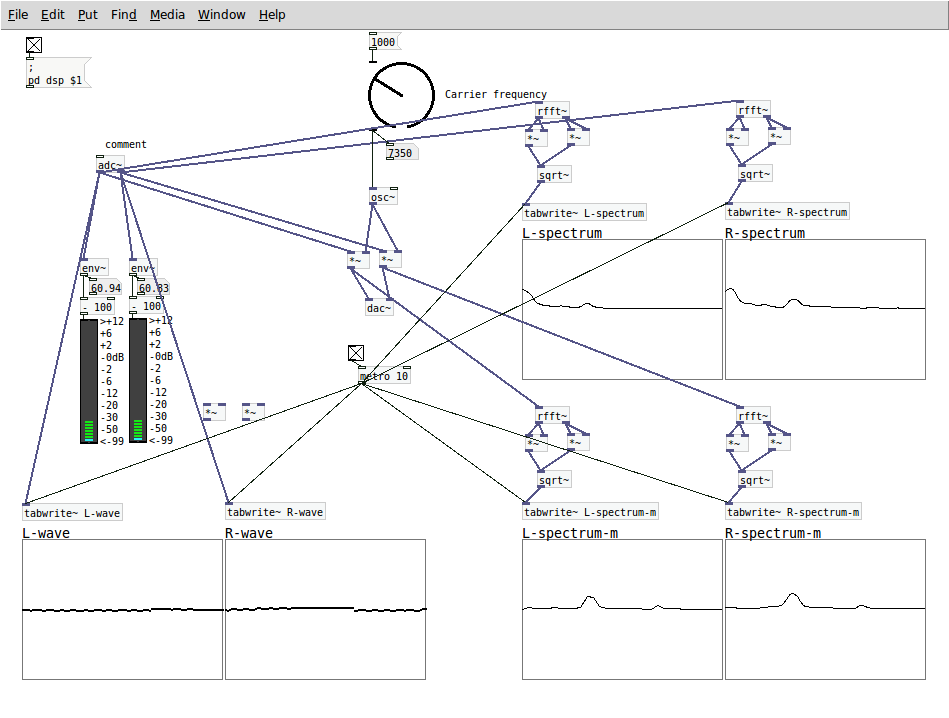
\includegraphics{amplitude-modulation-1}
\end{center}

\item Version 2 (using sends and receives):

\begin{verbatim}
cat > amplitude-modulation-2.pd << EOF
#N canvas 617 127 1154 962 10;
#X obj 94 -240 adc~;
#X obj 828 46 *~;
#X obj 860 45 *~;
#X obj 846 93 dac~;
#X obj 850 -18 osc~;
#X obj 78 -137 env~;
#X obj 127 -137 env~;
#X obj 79 -74 vu 15 120 empty empty -1 -8 0 10 -66577 -1 1 0;
#X obj 128 -75 vu 15 120 empty empty -1 -8 0 10 -66577 -1 1 0;
#X obj 127 -99 - 100;
#X obj 78 -98 - 100;
#X obj 15 -353 tgl 15 0 empty empty empty 17 7 0 10 -262144 -1 -1 1
1;
#X msg 15 -333 \; pd dsp \$1;
#X obj 223 107 tabwrite~ R-wave;
#X obj 20 108 tabwrite~ L-wave;
#N canvas 0 0 450 300 (subpatch) 0;
#X array L-wave 100 float 3;
#A 0 -5.96047e-07 -0.000107408 0.000123501 0.000132918 2.80142e-05
0.000281692 2.40803e-05 -0.000208616 -0.000202775 0.000151992 0.000205398
-0.000183702 -0.000294328 4.8995e-05 -0.000420213 -6.19888e-06 -0.000101566
-0.000219822 -0.000320792 -0.000690699 -0.000278592 -0.000164032 0.000139236
-0.000349045 -0.000146866 3.82662e-05 -5.13792e-05 8.97646e-05 -0.000333786
-0.000366092 -0.000171423 -0.000333548 -9.88245e-05 -0.000293374 -0.000428677
-0.000506759 -0.000342608 -0.000474215 -0.000311971 -0.000304222 -0.000426173
-0.000111461 -0.000185728 -0.00029254 -0.000502229 -0.000620365 -0.000219703
-0.000557303 -0.0008775 -0.00060463 -0.000949621 -0.000714779 -0.000823379
-0.000718236 -0.000561714 -0.000801921 -0.000694871 -0.000490665 -0.000412345
-0.000799418 -0.000520706 -0.000224948 -0.000247836 -0.000737906 -0.000796914
-0.000888229 -0.0010711 -0.00100029 -0.000889421 -0.000692725 -0.000931025
-0.00108337 -0.000770331 -0.000556469 -0.000853896 -0.00103295 -0.00110519
-0.00112593 -0.000694513 -0.000778318 -0.000909686 -0.00111175 -0.00128877
-0.000876546 -0.00068748 -0.00105345 -0.00111425 -0.00140011 -0.000926733
-0.000594616 -0.000602126 -0.00111318 -0.000897288 -0.000674009 -0.000750065
-0.000349402 -0.000814676 -0.000812531 -0.000852466 -0.000762582;
#X coords 0 1 99 -1 200 140 1;
#X restore 20 144 graph;
#N canvas 0 0 450 300 (subpatch) 0;
#X array R-wave 100 float 3;
#A 0 -6.98567e-05 -0.000249147 5.80549e-05 -0.000182271 -0.000317693
0.000222206 -2.96831e-05 -0.000311971 -0.000132561 4.48227e-05 0.000132561
-8.58307e-06 -0.00042057 -0.000250697 0.000125051 4.11272e-05 -5.04255e-05
-0.000157237 -0.000450969 -0.000454664 -0.000431657 0.000100613 -0.000128269
-0.000412464 -0.000261664 -1.56164e-05 0.000194192 0.000140786 -0.000353217
-0.000131965 0.00017333 -0.000229239 -4.41074e-05 -0.000206232 -0.000459909
-0.000434995 -0.000143051 -0.000127792 -0.000171542 -0.000579715 -0.000150442
-8.54731e-05 -7.21216e-05 -0.000386834 -0.000581265 -0.000254989 -0.000529647
-0.000409365 -0.000453115 -0.000855446 -0.000799894 -0.000755787 -0.000645042
-0.000667691 -0.000463486 -0.000617862 -0.000640631 -0.000308633 -0.000333309
-0.000792861 -0.000680208 -0.00023365 -0.000472069 -0.00037849 -0.00088191
-0.000935078 -0.000614405 -0.000995755 -0.000690341 -0.000495672 -0.00072062
-0.000949264 -0.000870824 -0.000456691 -0.000563383 -0.00102675 -0.00109518
-0.00101292 -0.000409961 -0.00080657 -0.0013442 -0.0010426 -0.00112629
-0.000958085 -0.000831962 -0.00118279 -0.000812411 -0.00130808 -0.00120866
-0.000943184 -0.000874281 -0.00117743 -0.00117898 -0.000871658 -0.000306845
-0.000781655 -0.000844479 -0.000691652 -0.0009166 -0.00090301;
#X coords 0 1 99 -1 200 140 1;
#X restore 223 144 graph;
#X obj 96 -355 tgl 15 0 empty empty empty 17 7 0 10 -262144 -1 -1 1
1;
#X obj 253 -242 rfft~;
#X obj 243 -214 *~;
#X obj 285 -215 *~;
#X obj 255 -178 sqrt~;
#X obj 268 -130 tabwrite~ L-spectrum;
#X obj 459 -244 rfft~;
#X obj 449 -216 *~;
#X obj 491 -217 *~;
#X obj 461 -180 sqrt~;
#X obj 471 -131 tabwrite~ R-spectrum;
#N canvas 0 0 450 300 (subpatch) 0;
#X array L-spectrum 32 float 5;
#A 0 0.0195442 0.00817593 0.00548782 0.00352542 0.00197952 0.00165914
0.00166075 0.000954338 0.000817258 0.00129113 0.00146072 0.00152881
0.00223816 0.00185242 0.000388151 0.00104445 0.00300843 0.00192705
0.000826185 0.000547419 0.00112846 0.00174496 0.000760889 0.00149756
0.000968246 0.00195259 0.00193626 0.00175719 0.000575282 0.00155285
0.0016394 8.09608e-05;
#X coords 0 1 31 -1 200 140 1;
#X restore 268 -94 graph;
#N canvas 0 0 450 300 (subpatch) 0;
#X array R-spectrum 32 float 5;
#A 0 0.0175533 0.00722562 0.0045235 0.00142838 0.00211134 0.00221599
0.00101493 0.000579066 0.00151707 0.00053408 0.00106531 0.000938519
0.00432546 0.0020301 0.000585151 0.00112467 0.00336951 0.000863056
0.00111727 0.00113411 0.000592928 0.00251454 0.000653159 0.00161542
0.00213387 0.000865938 0.000550404 0.00127678 0.000472236 0.000717838
0.000716469 0.000725959;
#X coords 0 1 31 -1 200 140 1;
#X restore 471 -94 graph;
#X obj 481 84 rfft~;
#X obj 471 112 *~;
#X obj 513 111 *~;
#X obj 483 148 sqrt~;
#N canvas 0 0 450 300 (subpatch) 0;
#X array L-spectrum-modulated 32 float 1;
#A 0 0.00219504 0.0014184 0.00105871 0.000580603 0.00125773 0.00191861
0.000814898 0.00082533 0.00120923 0.0014777 0.00152529 0.00349748 0.00994944
0.00619251 0.00415783 0.000557319 0.00113695 0.00142816 0.00142593
0.000593171 0.000601995 0.000850319 0.00057299 0.000580439 0.000891542
0.00045952 0.00108085 0.00173529 0.00133119 0.000930282 0.0009818 0.000841899
;
#X coords 0 1 31 -1 200 140 1;
#X restore 483 236 graph;
#X obj 683 85 rfft~;
#X obj 673 113 *~;
#X obj 715 112 *~;
#X obj 685 149 sqrt~;
#N canvas 0 0 450 300 (subpatch) 0;
#X array R-spectrum-modulated 32 float 5;
#A 0 0.00406177 0.00131448 0.0006774 0.000166896 0.00128597 0.000777438
0.00146135 0.000787831 0.00172884 0.00152404 0.00187414 0.00332734
0.00814396 0.00398155 0.00276644 0.00115745 0.000941153 0.00100096
0.000736268 0.000316533 0.000800675 0.000380299 0.000580029 0.000898021
0.00193061 0.00194364 0.000532415 0.0006216 0.00186499 0.000261477
0.000675644 0.000803884;
#X coords 0 1 31 -1 200 140 1;
#X restore 686 236 graph;
#X text 863 -45 Carrier frequency;
#X floatatom 87 -117 5 0 0 0 - - -;
#X floatatom 135 -117 5 0 0 0 - - -;
#X floatatom 867 -62 5 0 0 0 - - -;
#X msg 850 -173 1000;
#X obj 850 -142 knob 64 64 0 22050 0 0 empty empty empty 0 -8 0 8 -260097
-1 -1 2400 1;
#X text 101 -261 comment;
#X obj 33 -215 s~ L-channel;
#X obj 21 62 r~ L-channel;
#X obj 30 -165 r~ L-channel;
#X obj 774 18 r~ L-channel;
#X obj 253 -290 r~ L-channel;
#X obj 117 -216 s~ R-channel;
#X obj 127 -165 r~ R-channel;
#X obj 224 62 r~ R-channel;
#X obj 860 18 r~ R-channel;
#X obj 459 -292 r~ R-channel;
#X obj 106 -304 s metro;
#X obj 35 86 r metro;
#X obj 236 84 r metro;
#X obj 496 173 r metro;
#X obj 699 172 r metro;
#X obj 283 -155 r metro;
#X obj 488 -155 r metro;
#X obj 483 199 tabwrite~ L-spectrum-modulated;
#X obj 686 200 tabwrite~ R-spectrum-modulated;
#X obj 106 -334 metro 50;
#X connect 0 0 47 0;
#X connect 0 1 52 0;
#X connect 1 0 3 0;
#X connect 1 0 30 0;
#X connect 2 0 3 1;
#X connect 2 0 35 0;
#X connect 4 0 1 1;
#X connect 4 0 2 1;
#X connect 5 0 10 0;
#X connect 5 0 41 0;
#X connect 6 0 9 0;
#X connect 6 0 42 0;
#X connect 9 0 8 0;
#X connect 10 0 7 0;
#X connect 11 0 12 0;
#X connect 17 0 66 0;
#X connect 18 0 19 0;
#X connect 18 0 19 1;
#X connect 18 1 20 0;
#X connect 18 1 20 1;
#X connect 19 0 21 0;
#X connect 20 0 21 0;
#X connect 21 0 22 0;
#X connect 23 0 24 0;
#X connect 23 0 24 1;
#X connect 23 1 25 0;
#X connect 23 1 25 1;
#X connect 24 0 26 0;
#X connect 25 0 26 0;
#X connect 26 0 27 0;
#X connect 30 0 31 0;
#X connect 30 0 31 1;
#X connect 30 1 32 0;
#X connect 30 1 32 1;
#X connect 31 0 33 0;
#X connect 32 0 33 0;
#X connect 33 0 64 0;
#X connect 35 0 36 0;
#X connect 35 0 36 1;
#X connect 35 1 37 0;
#X connect 35 1 37 1;
#X connect 36 0 38 0;
#X connect 37 0 38 0;
#X connect 38 0 65 0;
#X connect 44 0 45 0;
#X connect 45 0 43 0;
#X connect 45 0 4 0;
#X connect 48 0 14 0;
#X connect 49 0 5 0;
#X connect 50 0 1 0;
#X connect 51 0 18 0;
#X connect 53 0 6 0;
#X connect 54 0 13 0;
#X connect 55 0 2 0;
#X connect 56 0 23 0;
#X connect 58 0 14 0;
#X connect 59 0 13 0;
#X connect 60 0 64 0;
#X connect 61 0 65 0;
#X connect 62 0 22 0;
#X connect 63 0 27 0;
#X connect 66 0 57 0;
EOF

pd-extended amplitude-modulation-2.pd &
\end{verbatim}

\begin{center}
  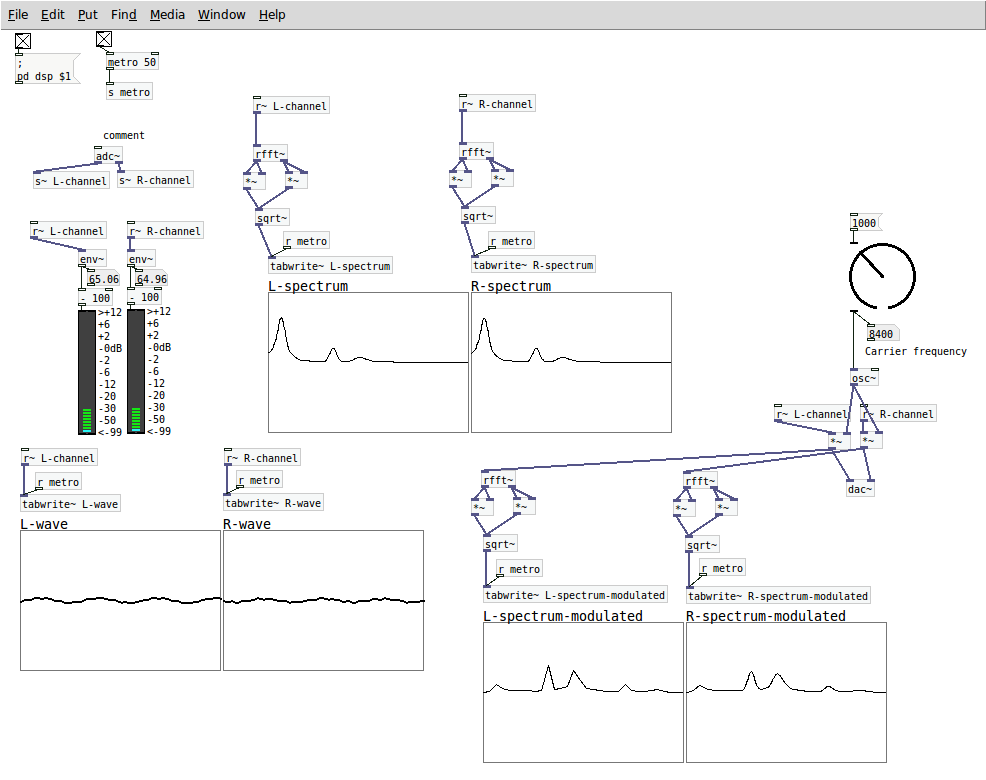
\includegraphics{amplitude-modulation-2}
\end{center}

\item Version 3 (using subpatching):

\begin{verbatim}
cat > amplitude-modulation-3.pd << EOF
#N canvas 615 81 1154 962 10;
#X obj 94 -240 adc~;
#X obj 663 17 *~;
#X obj 695 16 *~;
#X obj 681 64 dac~;
#X obj 685 -47 osc~;
#X obj 78 -137 env~;
#X obj 127 -137 env~;
#X obj 79 -74 vu 15 120 empty empty -1 -8 0 10 -66577 -1 1 0;
#X obj 128 -75 vu 15 120 empty empty -1 -8 0 10 -66577 -1 1 0;
#X obj 127 -99 - 100;
#X obj 78 -98 - 100;
#X obj 15 -353 tgl 15 0 empty empty empty 17 7 0 10 -262144 -1 -1 0
1;
#X msg 15 -333 \; pd dsp \$1;
#X obj 223 107 tabwrite~ R-wave;
#X obj 20 108 tabwrite~ L-wave;
#N canvas 0 0 450 300 (subpatch) 0;
#X array L-wave 100 float 3;
#A 0 -0.000231385 -0.000319004 -0.000555515 -0.000437021 9.13143e-05
-0.000187159 -0.000225186 0.000345111 0.000179052 0.000228643 1.88351e-05
2.07424e-05 0.000108361 0.000291467 0.00050509 0.000445843 0.000516295
6.91414e-06 0.000363588 0.000561833 0.000721932 0.000422239 -6.42538e-05
0.0001266 0.000448823 -0.000100613 -0.000260711 -0.000201583 -0.000144362
-0.000462771 -0.000640035 -0.000618935 -0.000422359 -0.000273466 -0.000565171
-0.000524998 -0.000305533 -0.000240564 -0.000421763 -0.0006181 -0.000558853
-0.000553012 -0.000856161 -0.000363827 -7.76053e-05 -0.000295043 -0.000331163
-0.000188112 -0.000537038 -0.000523567 -0.000597835 -0.000456572 -0.000149369
-0.000326753 -0.000404835 -0.000282645 -0.000320673 -0.000473261 -0.000627637
-0.000270844 -0.00035274 -0.000459433 -0.000648141 -0.000508785 -0.000312209
-0.000733614 -0.00112832 -0.000754237 -0.000633836 -0.000402927 -0.000477195
-0.000286341 -3.25441e-05 -0.000591397 -0.000722885 -0.000430942 -0.000270605
-0.000486016 -0.000867367 -0.000529528 -0.000460744 -0.000212669 -0.000370979
-7.71284e-05 -0.000185847 -0.000315547 -0.000399351 -0.000282884 -0.000130296
-0.000160694 -0.000126362 -0.000187397 -0.000194907 -0.000206351 -0.000347376
-0.000263453 -0.000251889 -0.000423551 -0.000200272 -0.0001086;
#X coords 0 1 99 -1 200 140 1;
#X restore 20 144 graph;
#N canvas 0 0 450 300 (subpatch) 0;
#X array R-wave 100 float 3;
#A 0 -0.000347495 -0.000257731 -0.000621915 -0.000511169 -0.000177264
1.5378e-05 -0.000175357 2.31266e-05 0.000253916 3.93391e-06 -0.000175357
-0.000104785 9.17912e-05 9.35793e-05 0.000173688 0.000171781 0.00012207
7.05719e-05 0.000125885 0.000366211 0.000633121 0.000400305 0.000220895
0.000173211 0.000182629 -0.000137806 -0.000282764 -0.000282645 4.1604e-05
-0.000465751 -0.000608683 -0.000276685 -0.000501633 -0.000305057 -0.000524283
-0.000535607 -0.000266552 -0.000337124 -0.000260711 -0.000733614 -0.000472188
-0.000416756 -0.000403285 -0.000616789 -0.000431657 -0.000170231 -0.000349522
-0.000404716 -0.000227213 -0.000438929 -0.000633359 -0.000495911 -0.000291705
-0.000327826 -0.000295281 -0.000650048 -0.000363708 -0.000493407 -0.000575304
-0.00049305 -0.000479579 -0.000506163 -0.000704408 -0.000416279 -0.000376105
-0.000580072 -0.000822187 -0.000572205 -0.000402212 -0.000453711 -0.000445962
-0.000209332 0.000116944 -0.000111938 -0.000464797 -0.000228167 -0.000336885
-0.000430226 -0.000548363 -0.000546336 -7.31945e-05 -0.000294447 -0.000248551
5.66244e-05 -6.73533e-05 -4.82798e-05 -0.000261903 -3.09944e-05 -3.29018e-05
-0.000303745 -0.000162482 -0.000450492 3.02792e-05 -5.96047e-06 -0.000240564
-0.000219584 -0.000253797 -0.000185132 -9.34601e-05 -0.000490189;
#X coords 0 1 99 -1 200 140 1;
#X restore 223 144 graph;
#X obj 96 -355 tgl 15 0 empty empty empty 17 7 0 10 -262144 -1 -1 1
1;
#X obj 230 -230 tabwrite~ L-spectrum;
#X obj 433 -231 tabwrite~ R-spectrum;
#N canvas 0 0 450 300 (subpatch) 0;
#X array L-spectrum 32 float 5;
#A 0 0.0125817 0.0119714 0.00736391 0.00111757 0.00196076 0.00186084
0.0013529 0.00224929 0.00196935 0.00071846 0.00244962 0.00155824 0.000662175
0.00177553 0.00236652 0.000900354 0.00428685 0.000434677 0.000374034
0.00149237 0.0011689 0.00123219 0.00129497 0.00147874 0.000555072 0.000538826
0.000652727 0.0014933 0.000841224 0.000361149 0.000638969 0.000947994
;
#X coords 0 1 31 -1 200 140 1;
#X restore 230 -194 graph;
#N canvas 0 0 450 300 (subpatch) 0;
#X array R-spectrum 32 float 5;
#A 0 0.0153836 0.0101812 0.00577934 0.00131737 0.00251711 0.00203522
0.000315623 0.000782838 0.0020434 0.00115641 0.00174393 0.000882506
0.00112287 0.00081443 0.00163909 0.00085469 0.00323237 0.00155087 0.000695748
0.00141265 0.000520526 0.000459498 0.00106057 0.0007225 0.00044635
0.00115913 0.000707579 0.000920909 0.00158063 0.000408492 0.00078321
0.000716307;
#X coords 0 1 31 -1 200 140 1;
#X restore 433 -194 graph;
#N canvas 0 0 450 300 (subpatch) 0;
#X array L-spectrum-modulated 32 float 1;
#A 0 3.8041e-05 0.000547192 0.00144994 0.00184407 0.00167551 0.000692077
0.00495094 0.00609223 0.00668787 0.00649782 0.00334426 0.00102872 0.000526081
0.00110091 0.000947837 0.00199104 0.0011231 0.000622475 0.0011442 0.000491187
0.000480391 0.000943874 0.000999426 0.000845963 0.0022002 0.000669971
0.000138072 0.000740563 0.000995444 0.00125778 0.00049642 0.000679238
;
#X coords 0 1 31 -1 200 140 1;
#X restore 563 151 graph;
#N canvas 0 0 450 300 (subpatch) 0;
#X array R-spectrum-modulated 32 float 5;
#A 0 0.000303777 0.000405776 0.000995049 0.00182215 0.00128789 0.000617809
0.00377505 0.00532228 0.00842025 0.00604103 0.00210529 0.000622102
0.000779807 0.00106154 0.000941176 0.000386193 0.00121827 0.0011692
0.000695059 0.000889522 0.00129267 0.00046022 0.000629959 0.000784604
0.00179483 0.000420999 0.000870367 0.0004628 0.00134199 0.000437177
0.000869802 0.000735404;
#X coords 0 1 31 -1 200 140 1;
#X restore 766 151 graph;
#X text 698 -74 Carrier frequency;
#X floatatom 87 -117 5 0 0 0 - - -;
#X floatatom 135 -117 5 0 0 0 - - -;
#X floatatom 702 -91 5 0 0 0 - - -;
#X msg 685 -202 1000;
#X obj 685 -171 knob 64 64 0 22050 0 0 empty empty empty 0 -8 0 8 -260097
-1 -1 1600 1;
#X text 101 -261 comment;
#X obj 33 -215 s~ L-channel;
#X obj 21 62 r~ L-channel;
#X obj 30 -165 r~ L-channel;
#X obj 609 -11 r~ L-channel;
#X obj 229 -301 r~ L-channel;
#X obj 117 -216 s~ R-channel;
#X obj 127 -165 r~ R-channel;
#X obj 224 62 r~ R-channel;
#X obj 695 -11 r~ R-channel;
#X obj 432 -304 r~ R-channel;
#X obj 106 -304 s metro;
#X obj 35 86 r metro;
#X obj 236 84 r metro;
#X obj 576 88 r metro;
#X obj 779 87 r metro;
#X obj 245 -255 r metro;
#X obj 450 -255 r metro;
#X obj 563 114 tabwrite~ L-spectrum-modulated;
#X obj 766 115 tabwrite~ R-spectrum-modulated;
#X obj 106 -334 metro 50;
#N canvas 320 744 316 392 spectrum 0;
#X obj 57 71 rfft~;
#X obj 47 99 *~;
#X obj 89 98 *~;
#X obj 59 135 sqrt~;
#X obj 59 168 outlet~;
#X obj 57 39 inlet~;
#X connect 0 0 1 0;
#X connect 0 0 1 1;
#X connect 0 1 2 0;
#X connect 0 1 2 1;
#X connect 1 0 3 0;
#X connect 2 0 3 0;
#X connect 3 0 4 0;
#X connect 5 0 0 0;
#X restore 229 -276 pd spectrum;
#N canvas 320 744 316 392 spectrum 0;
#X obj 57 71 rfft~;
#X obj 47 99 *~;
#X obj 89 98 *~;
#X obj 59 135 sqrt~;
#X obj 59 168 outlet~;
#X obj 57 39 inlet~;
#X connect 0 0 1 0;
#X connect 0 0 1 1;
#X connect 0 1 2 0;
#X connect 0 1 2 1;
#X connect 1 0 3 0;
#X connect 2 0 3 0;
#X connect 3 0 4 0;
#X connect 5 0 0 0;
#X restore 432 -280 pd spectrum;
#N canvas 320 744 316 392 spectrum 0;
#X obj 57 71 rfft~;
#X obj 47 99 *~;
#X obj 89 98 *~;
#X obj 59 135 sqrt~;
#X obj 59 168 outlet~;
#X obj 57 39 inlet~;
#X connect 0 0 1 0;
#X connect 0 0 1 1;
#X connect 0 1 2 0;
#X connect 0 1 2 1;
#X connect 1 0 3 0;
#X connect 2 0 3 0;
#X connect 3 0 4 0;
#X connect 5 0 0 0;
#X restore 563 60 pd spectrum;
#N canvas 320 744 316 392 spectrum 0;
#X obj 57 71 rfft~;
#X obj 47 99 *~;
#X obj 89 98 *~;
#X obj 59 135 sqrt~;
#X obj 59 168 outlet~;
#X obj 57 39 inlet~;
#X connect 0 0 1 0;
#X connect 0 0 1 1;
#X connect 0 1 2 0;
#X connect 0 1 2 1;
#X connect 1 0 3 0;
#X connect 2 0 3 0;
#X connect 3 0 4 0;
#X connect 5 0 0 0;
#X restore 766 62 pd spectrum;
#X connect 0 0 31 0;
#X connect 0 1 36 0;
#X connect 1 0 3 0;
#X connect 1 0 53 0;
#X connect 2 0 3 1;
#X connect 2 0 54 0;
#X connect 4 0 1 1;
#X connect 4 0 2 1;
#X connect 5 0 10 0;
#X connect 5 0 25 0;
#X connect 6 0 9 0;
#X connect 6 0 26 0;
#X connect 9 0 8 0;
#X connect 10 0 7 0;
#X connect 11 0 12 0;
#X connect 17 0 50 0;
#X connect 28 0 29 0;
#X connect 29 0 27 0;
#X connect 29 0 4 0;
#X connect 32 0 14 0;
#X connect 33 0 5 0;
#X connect 34 0 1 0;
#X connect 35 0 51 0;
#X connect 37 0 6 0;
#X connect 38 0 13 0;
#X connect 39 0 2 0;
#X connect 40 0 52 0;
#X connect 42 0 14 0;
#X connect 43 0 13 0;
#X connect 44 0 48 0;
#X connect 45 0 49 0;
#X connect 46 0 18 0;
#X connect 47 0 19 0;
#X connect 50 0 41 0;
#X connect 51 0 18 0;
#X connect 52 0 19 0;
#X connect 53 0 48 0;
#X connect 54 0 49 0;
EOF

pd-extended amplitude-modulation-3.pd &
\end{verbatim}

\begin{center}
  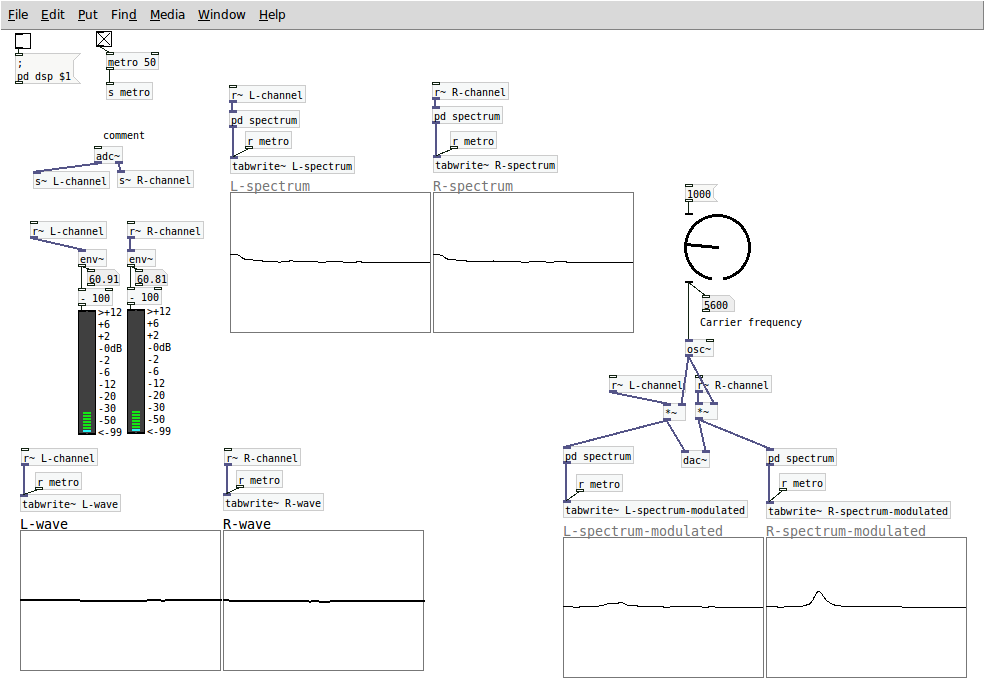
\includegraphics{amplitude-modulation-3}
\end{center}

\end{itemize}

% 1. Lanzar JACK usando qjackctl y ejecutar el demonio.
% 2. Lanzar amsynth. Debería aparecer una MIDI Writable Clients "amsynth" y una ALSA Writable Clients "amSynth".
% 3. Lanzar Pure Data (pd-extended).
% 4. En Pure Data seleccionar en la pestaña de Media: jack y ALSA-MIDI.
% 5. Comprobar que entre las conexiones ALSA controladas por JACK, Pure Data se conecta con amSynth.
% 6. Ejecutar PD->Media->Test Audio and MIDI (pinchar en MIDI OUT).
